\begin{wrapfigure}{}{0.5\textwidth}
    % \begin{figure}[h]
    \begin{center}
        \includegraphics[width=0.45\textwidth]{../figures/final_dose_profile.pdf}
    \end{center}
        \caption{Dose profile utilized to create pillar waveguides using Medusa mask. The dose factor (DF) corresponding to each ring is shown on it.}
        \label{fig:final_dose_profile}
    % \end{figure}
\end{wrapfigure}

\begin{equation}\label{eq:sens_shot}
    \eta_{\text{AC}} \approx \frac{\pi}{2 \gamma_{\text{NV}} C \sqrt{T_2}},
\end{equation}

\begin{figure}[h]
    \centering 
    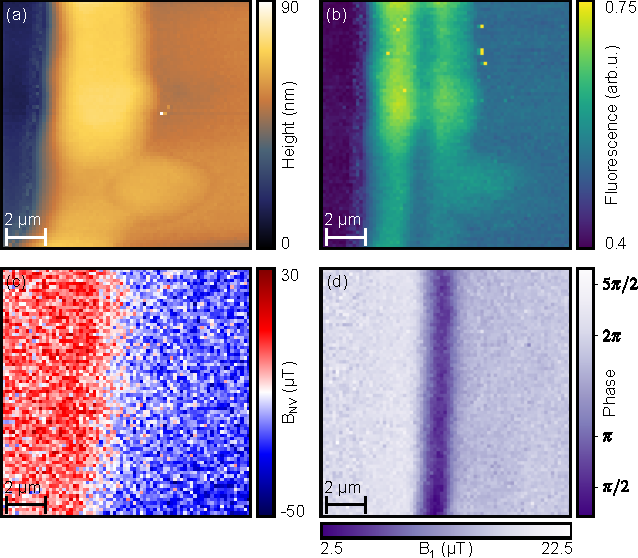
\includegraphics[width=0.95\textwidth]{../figures/grad_xy.pdf}
    \caption[Gradiometry spatial scan]{Gradiometry spatial scan. }
    \label{fig:grad_xy}
\end{figure}

\begin{equation}\label{eq:four_phase}
    \begin{split}
        \frac{C_{X}-C_{-X}}{C_{-Y}-C_{Y}} = \frac{2\sin\phi}{2\cos\phi} = \tan\phi \\
        \phi = \text{arctan}\left (\frac{C_{X}-C_{-X}}{C_{-Y}-C_{Y}} \right ).
    \end{split}
\end{equation}